\begin{pastexam}[label={px:gw3-104-ds-04}]{關務三等資訊處理 104 年 第四題}
（申論；20 分）

圖形的理論是起源於西元十八世紀，有一位數學家尤拉（Eular）為了解決「肯尼茲堡橋樑」問題，而想出的一種圖形結構理論。
所謂的「肯尼茲堡橋樑」問題是：某一個人由某地點出發，最後再回到原點，必須要經過每一座橋，並且只能經過一次。如下圖
所示：
\begin{center}
\begin{tikzpicture}[x=1cm,y=1cm,
  br/.style={line width=5.5pt, draw=black, postaction={draw=white, line width=4pt},
    postaction={draw=black, line width=4pt, dash pattern=on 0.5pt off 1.5pt}},
  num/.style={font=\small}]
\draw[thick] (-0.2,1.7) .. controls (1,1.3) and (2,2.3) .. (3.3,1.8) .. controls (4.5,1.3) and (5,2.2) .. (5.8,1.9);
\draw[thick] (0.3,-1.6) .. controls (1.5,-1.2) and (2.6,-2.0) .. (3.6,-1.6) .. controls (4.6,-1.2) and (5.4,-2.0) .. (6.0,-1.7);
\node at (1.75,2.25) {C};
\node at (2.0,-2.2) {B};
\draw[br] (1.0,1.55) -- (1.55,0.15);
\draw[br] (2.65,1.75) -- (2.05,0.15);
\draw[br] (5.0,1.75) -- (5.45,0.25);
\draw[br] (1.55,-0.15) -- (0.95,-1.5);
\draw[br] (2.05,-0.15) -- (2.7,-1.65);
\draw[br] (5.45,-0.3) -- (5.15,-1.6);
\draw[br] (2.8,0) -- (4.3,0);
\draw[thick,fill=white] (1.8,0) ellipse (1.05 and 0.42);
\draw[thick,fill=white] (5.2,0) ellipse (0.95 and 0.42);
\node at (1.8,0.12) {A};
\node[font=\tiny] at (1.8,-0.15) {肯尼茲堡};
\node at (5.6,0.05) {D};
\node[num] at (0.85,0.95) {3};
\node[num] at (2.72,1.0) {4};
\node[num] at (3.55,0.25) {5};
\node[num] at (5.6,1.25) {6};
\node[num] at (0.95,-0.75) {1};
\node[num] at (2.15,-0.95) {2};
\node[num] at (5.55,-0.95) {7};
\end{tikzpicture}
\end{center}
\begin{itemize}[leftmargin=2.2em, nosep]
\item[㈠] 請問肯尼茲堡的人有無可能走過所有的橋樑 1 次，到過每個地方，而後又回到肯尼茲堡？（5 分）
\item[㈡] 土地代表頂點 A,B,C,D，橋樑代表邊 1\textasciitilde 7，請畫出此圖形結構。（5 分）
\item[㈢] 數學家尤拉（Eular）對「肯尼茲堡橋樑」問題所找出的規則是什麼？（5 分）
\item[㈣] 請舉一個具有尤拉循環（Eulerian Cycle）的例子，並寫出其路徑。（5 分）
\end{itemize}
\end{pastexam}

\begin{pastsoln}
答案：㈠ 不可能。 ㈡ 圖在下面（A 度數 $5$，B、C、D 度數 $3$）。 ㈢ 連通圖有尤拉循環若且唯若每個頂點的度數都是偶數。
㈣ 例子和路徑在下面。

原卷「Eular」是 Euler 的誤拼。 肯尼茲堡（Königsberg）現在多譯作哥尼斯堡。

\textbf{㈡ 圖形結構。} 土地是頂點、橋是邊；兩塊土地之間有兩座橋就畫兩條邊，所以這是\textbf{多重圖}（multigraph）。
從圖上讀出：橋 1、2 連 A--B，橋 3、4 連 A--C，橋 5 連 A--D，橋 6 連 C--D，橋 7 連 B--D。
\begin{center}
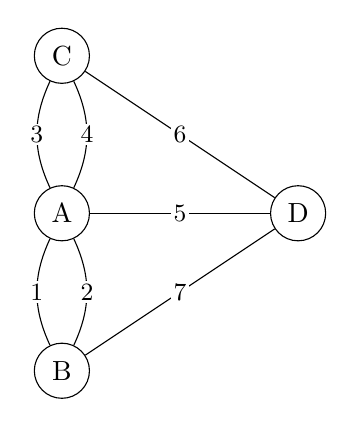
\begin{tikzpicture}[v/.style={circle,draw,minimum size=7mm,inner sep=0pt}, lab/.style={font=\small,fill=white,inner sep=1pt}]
\node[v] (C) at (0,2) {C};
\node[v] (A) at (0,0) {A};
\node[v] (B) at (0,-2) {B};
\node[v] (D) at (3,0) {D};
\draw (A) to[bend left=25] node[lab] {3} (C);
\draw (A) to[bend right=25] node[lab] {4} (C);
\draw (A) to[bend right=25] node[lab] {1} (B);
\draw (A) to[bend left=25] node[lab] {2} (B);
\draw (A) -- node[lab] {5} (D);
\draw (C) -- node[lab] {6} (D);
\draw (B) -- node[lab] {7} (D);
\end{tikzpicture}
\end{center}
度數：$\deg A = 5$（1、2、3、4、5），$\deg B = 3$（1、2、7），$\deg C = 3$（3、4、6），$\deg D = 3$（5、6、7）。

\textbf{㈢ 尤拉的規則}（資結書第~21.7~節、定理~21.11）：
\begin{itemize}
\item 連通的（多重）圖有\textbf{尤拉循環}（每條邊恰走一次、回到起點）若且唯若\textbf{每個頂點的度數都是偶數}。
\item 連通圖有\textbf{尤拉路徑}（每條邊恰走一次、不必回到起點）若且唯若度數為奇數的頂點有 $0$ 個或 $2$ 個；有 $2$ 個時，
路徑必須從其中一個出發、在另一個結束。
\end{itemize}
理由：走過一個頂點（不是起點也不是終點）時，一定是走一條邊進來、再走另一條邊出去，每經過一次用掉兩條邊；起點和終點
相同時起點也是一出一進，所以每個頂點的度數都得是偶數。 反過來，度數全為偶數時可以用 Hierholzer 的方法把一個個迴圈
接起來，構造出尤拉循環（資結書虛擬碼~21.7）。

\textbf{㈠} 不可能。 四個頂點的度數 $5, 3, 3, 3$ 全是奇數，不符合尤拉循環的條件，連尤拉路徑（不回原點）的條件
「奇數度頂點 $0$ 或 $2$ 個」也不符合。 所以從肯尼茲堡出發，不可能每座橋恰走一次再回到肯尼茲堡。

\textbf{㈣ 例子。} 最簡單的例子是三角形：頂點 $X, Y, Z$，邊 $XY, YZ, ZX$，每個頂點度數 $2$，尤拉循環
$X \to Y \to Z \to X$。 和本題相關的例子：在肯尼茲堡再加兩座橋，橋 8 連 B--C、橋 9 連 A--D。 度數變成
$A = 6$、$B = 4$、$C = 4$、$D = 4$，全是偶數，圖連通，所以有尤拉循環，例如從 A 出發：
\[
A \xrightarrow{9} D \xrightarrow{7} B \xrightarrow{8} C \xrightarrow{6} D \xrightarrow{5} A \xrightarrow{4} C
\xrightarrow{3} A \xrightarrow{2} B \xrightarrow{1} A,
\]
九座橋各走一次，回到 A。
\end{pastsoln}
